\section{Digital Phantoms}\label{sect:digital_phantoms}

\subsection{Elastic Materials}
The first-phase of digital phantoms focused on ``simple'' elastic material
formulations with different focal configurations and stiffnesses to evaluate
shear wave speed reconstruction accuracy and precision without viscosity as a
confounding variable.

A nominal curvilinear array configuration was chosen for all of the simulations
(Table~\ref{table:curvilinear}).

\begin{table}[htb!]
    \centering
    \caption{Simulated Curvilinear Array Configuration}
    \begin{tabular}{|l|l|}
    \hline
    Radius of Curvature & 60 mm \\
    Element Height & 14 mm \\
    Element Pitch & 0.477 mm (0.007 mm kerf) \\
    Center Frequency & 3.0 MHz \\
    Fractional Bandwidth & 100\% \\
    Elevation Focus & 50 mm \\
    \hline
    \end{tabular}
\label{table:curvilinear}
\end{table}

The acoustic radiation force excitation was simulated with several focal configurations (Table~\ref{table:arf}).

\begin{table}[htb!]
    \centering
    \caption{Acoustic Radiation Force Focal Configurations}
    \begin{tabular}{|l|l|}
    \hline
    Frequency & 3.0 MHz \\
    F/\# & [2 ,3.5] \\
    Excitation Durations & [500, 1000] cycles \\
    Focal Depths & [30, 50 70] mm \\
    \hline
    \end{tabular}
\label{table:arf}
\end{table}

Field II~\cite{Jensen1992} was used to simulate the acoustic intensity
associated with the different acoustic radiation force transmit conditions.
The material was acoustically modeled as linear with a constant acoustic
attenuation of 0.45 dB/(cm $\cdot$ MHz).  The acoustic intensity was mapped at
locations in the finite element meshes and the radiation force was either
applied as a point load~\cite{Palmeri2005} at each nodal location or a body
force across elements.

Different elastic material properties were simulated for each of the different
acoustic radiation force focal configurations (Table~\ref{table:elastic}).

\begin{table}[htb!]
    \centering
    \caption{Elastic Material Properties}
    \begin{tabular}{|l|l|}
    \hline
    Poisson's Ratio & 0.495 \\
    Young's Moduli &  [1.0, 2.0, 5.0, 10.0] kPa \\
    \hline
    \end{tabular}
\label{table:elastic}
\end{table}

The finite mesh boundaries were either simulated having perfect matching layers
or infinite elements to reduce artifacts associated with compression and
shear wave reflections back into the regions of interest.  Different mesh densities were also studied to evaluate numerical accuracy; ultimately a uniform node spacing of 0.167 mm was used for the digital phantoms.

All of the model configuration scripts for LS-DYNA and ABAQUS have been uploaded to GitHub:

\url{https://github.com/RSNA-QIBA-US-SWS/QIBA-DigitalPhantoms/tree/master/dyna}\\
\url{https://github.com/RSNA-QIBA-US-SWS/QIBA-DigitalPhantoms/tree/master/abaqus}

All of the digital phantom data has been saved in Matlab format and uploaded as
a single archive to QIDW:

\url{http://qidw.rsna.org/community/14}:\verb+US-SWS-Digital-Phantoms -> Public ->+\\
\verb+Elastic Digital Phantoms -> ElasticDigitalPhantomDataMesh0p167mm.zip+

A comprehensive comparison of LS-DYNA and ABAQUS results has been performed
and the corresponding code to process the data are available on GitHub:

\url{https://github.com/RSNA-QIBA-US-SWS/QIBA-DigitalPhantoms/tree/master/results}

\subsection{Viscoelastic Materials}

\begin{figure}[htb!]
    \centering
    \begin{tabular}{c}
        $G_0$ = 10.0 kPa, $G_\infty$ = 2.0 kPa, $\beta$ = 6666.7 Pa$\cdot$s\\
        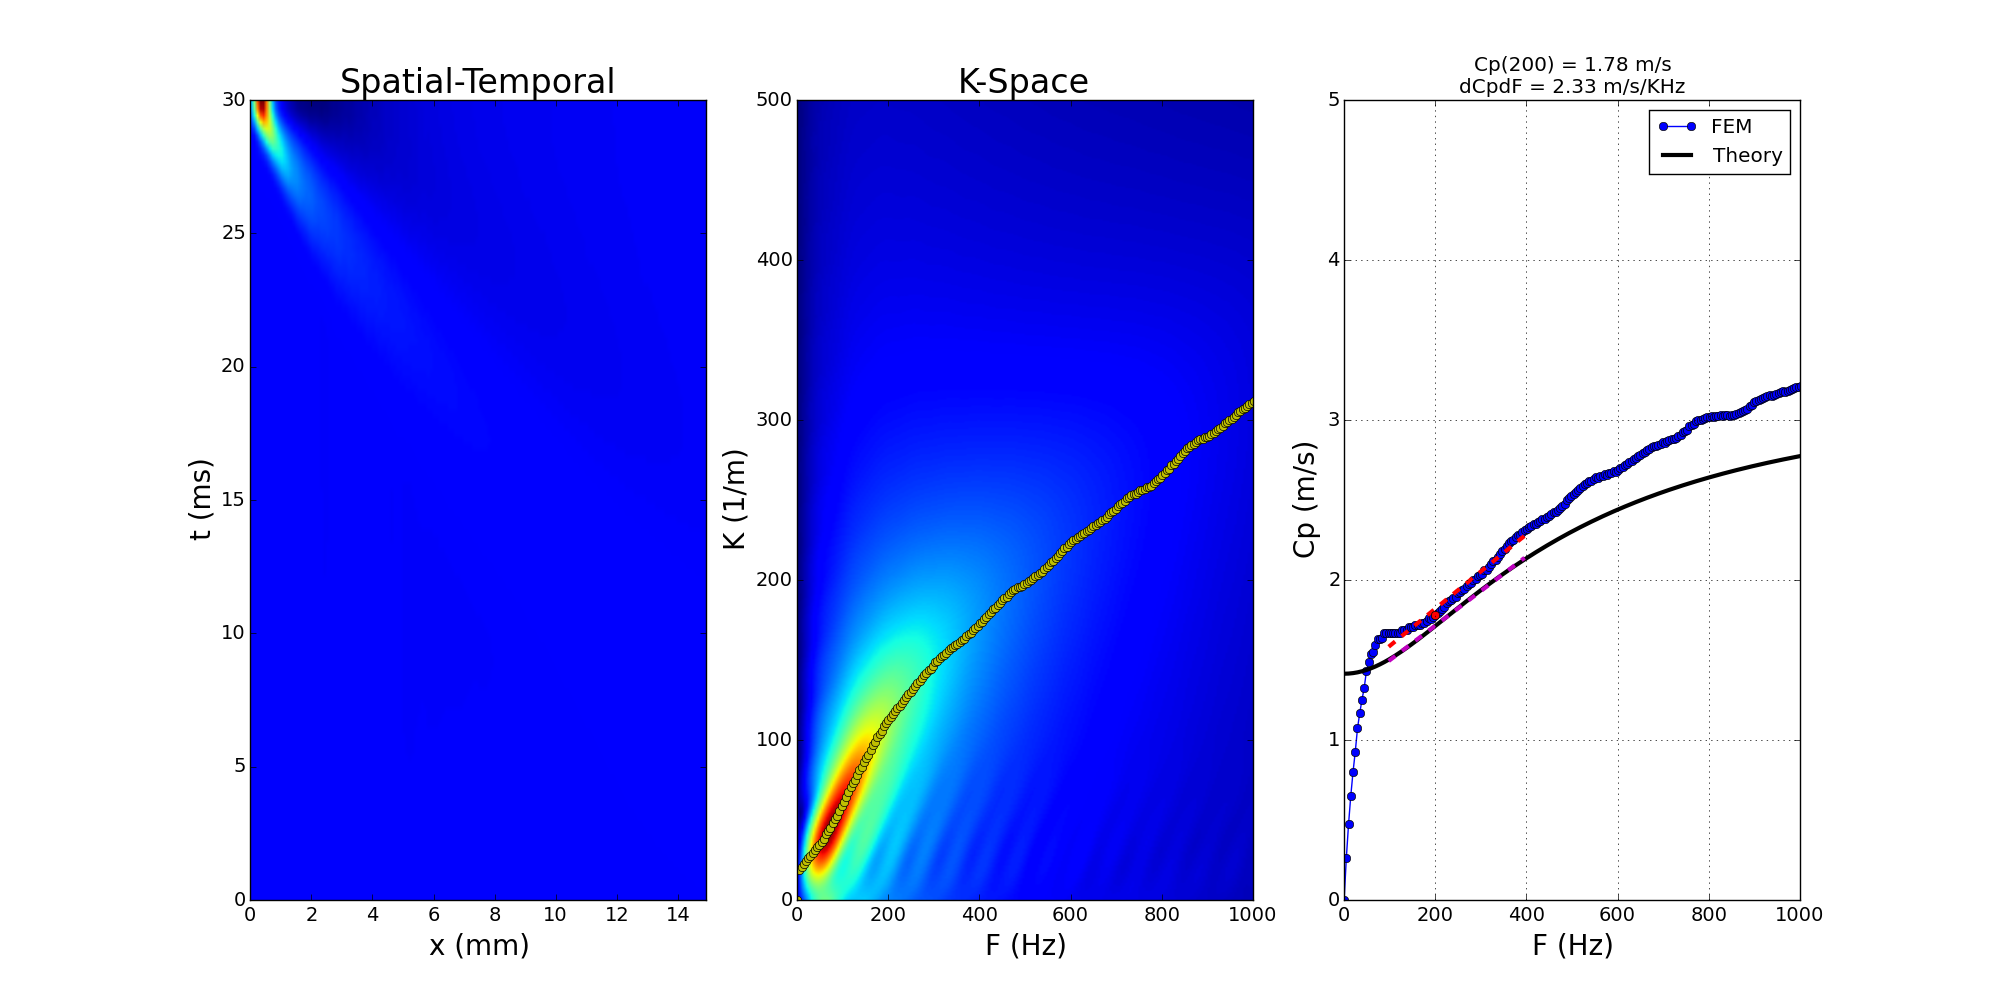
\includegraphics[width=0.75\linewidth]{figs/G010kPa_GI2kPa_BETA6667.png}\\
        $G_0$ = 15.0 kPa, $G_\infty$ = 4.0 kPa, $\beta$ = 5500.0 Pa$\cdot$s\\
        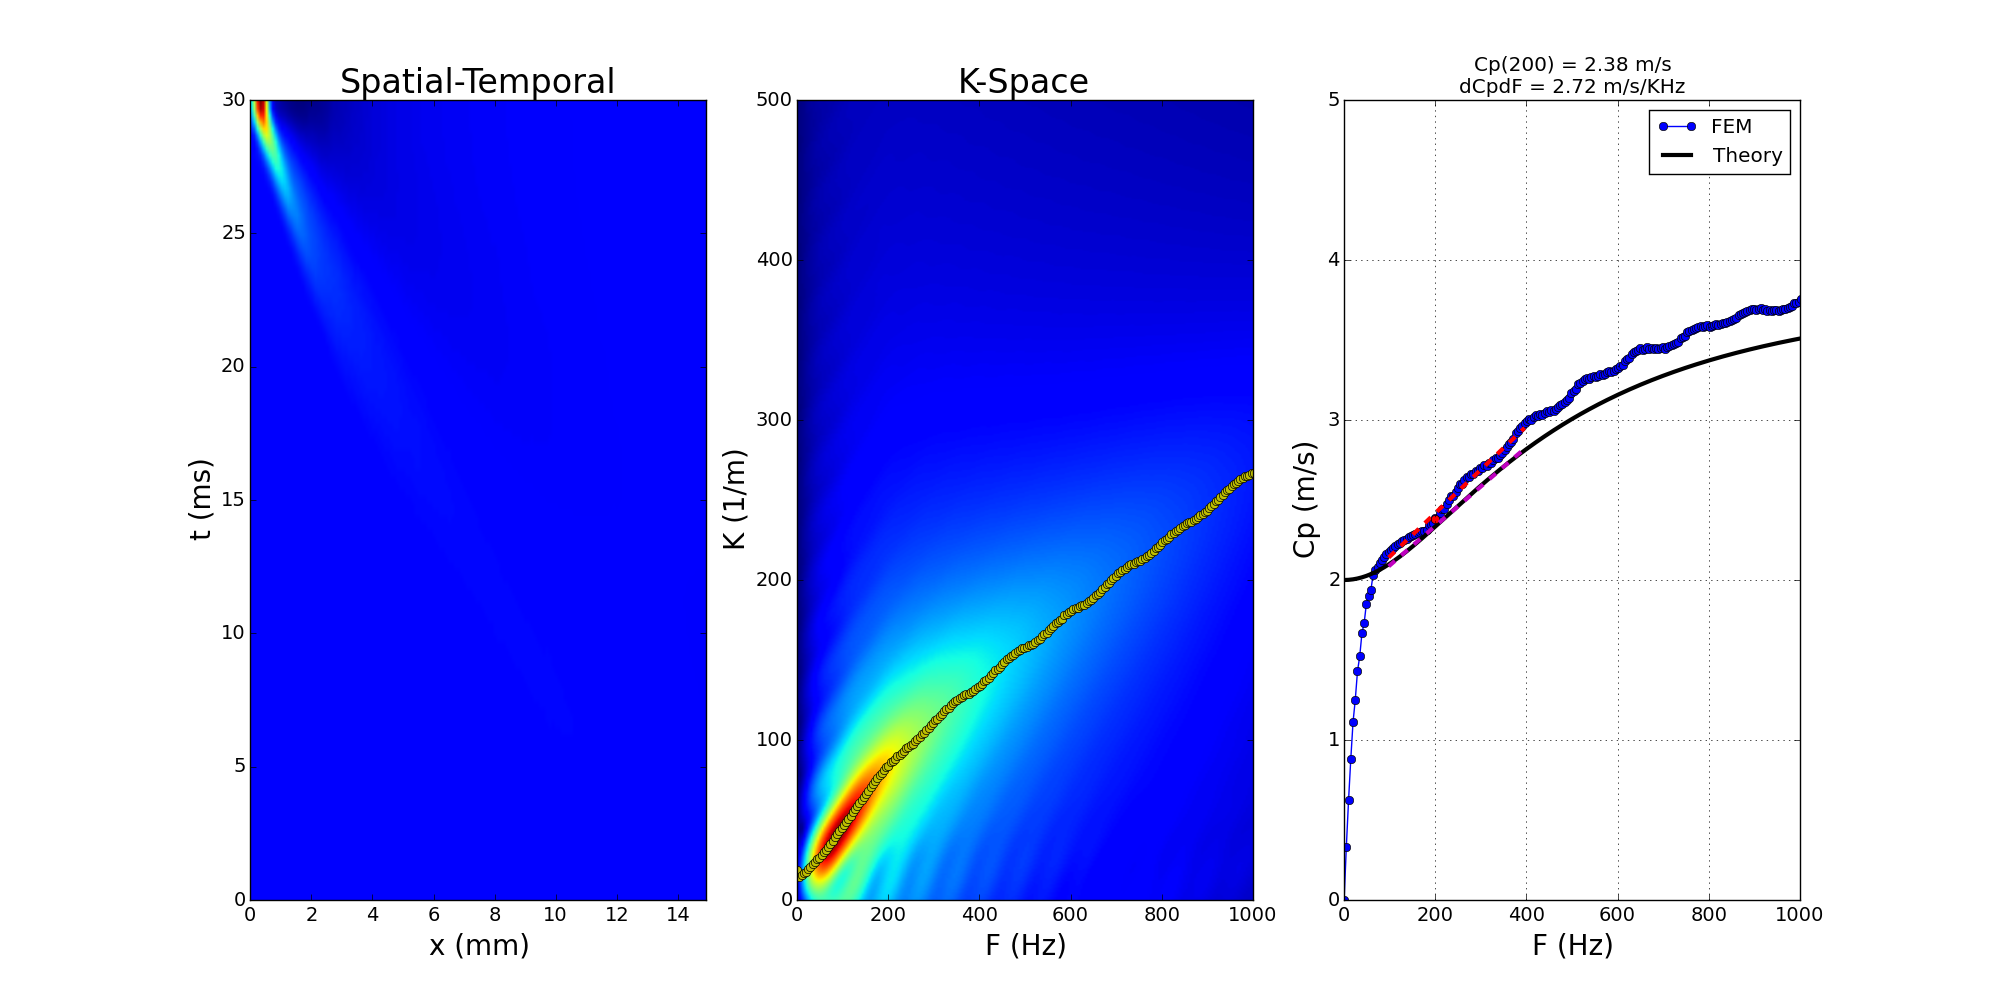
\includegraphics[width=0.75\linewidth]{figs/G015kPa_GI4kPa_BETA5500.png}\\
        $G_0$ = 20.0 kPa, $G_\infty$ = 4.0 kPa, $\beta$ = 4000.0 Pa$\cdot$s\\
        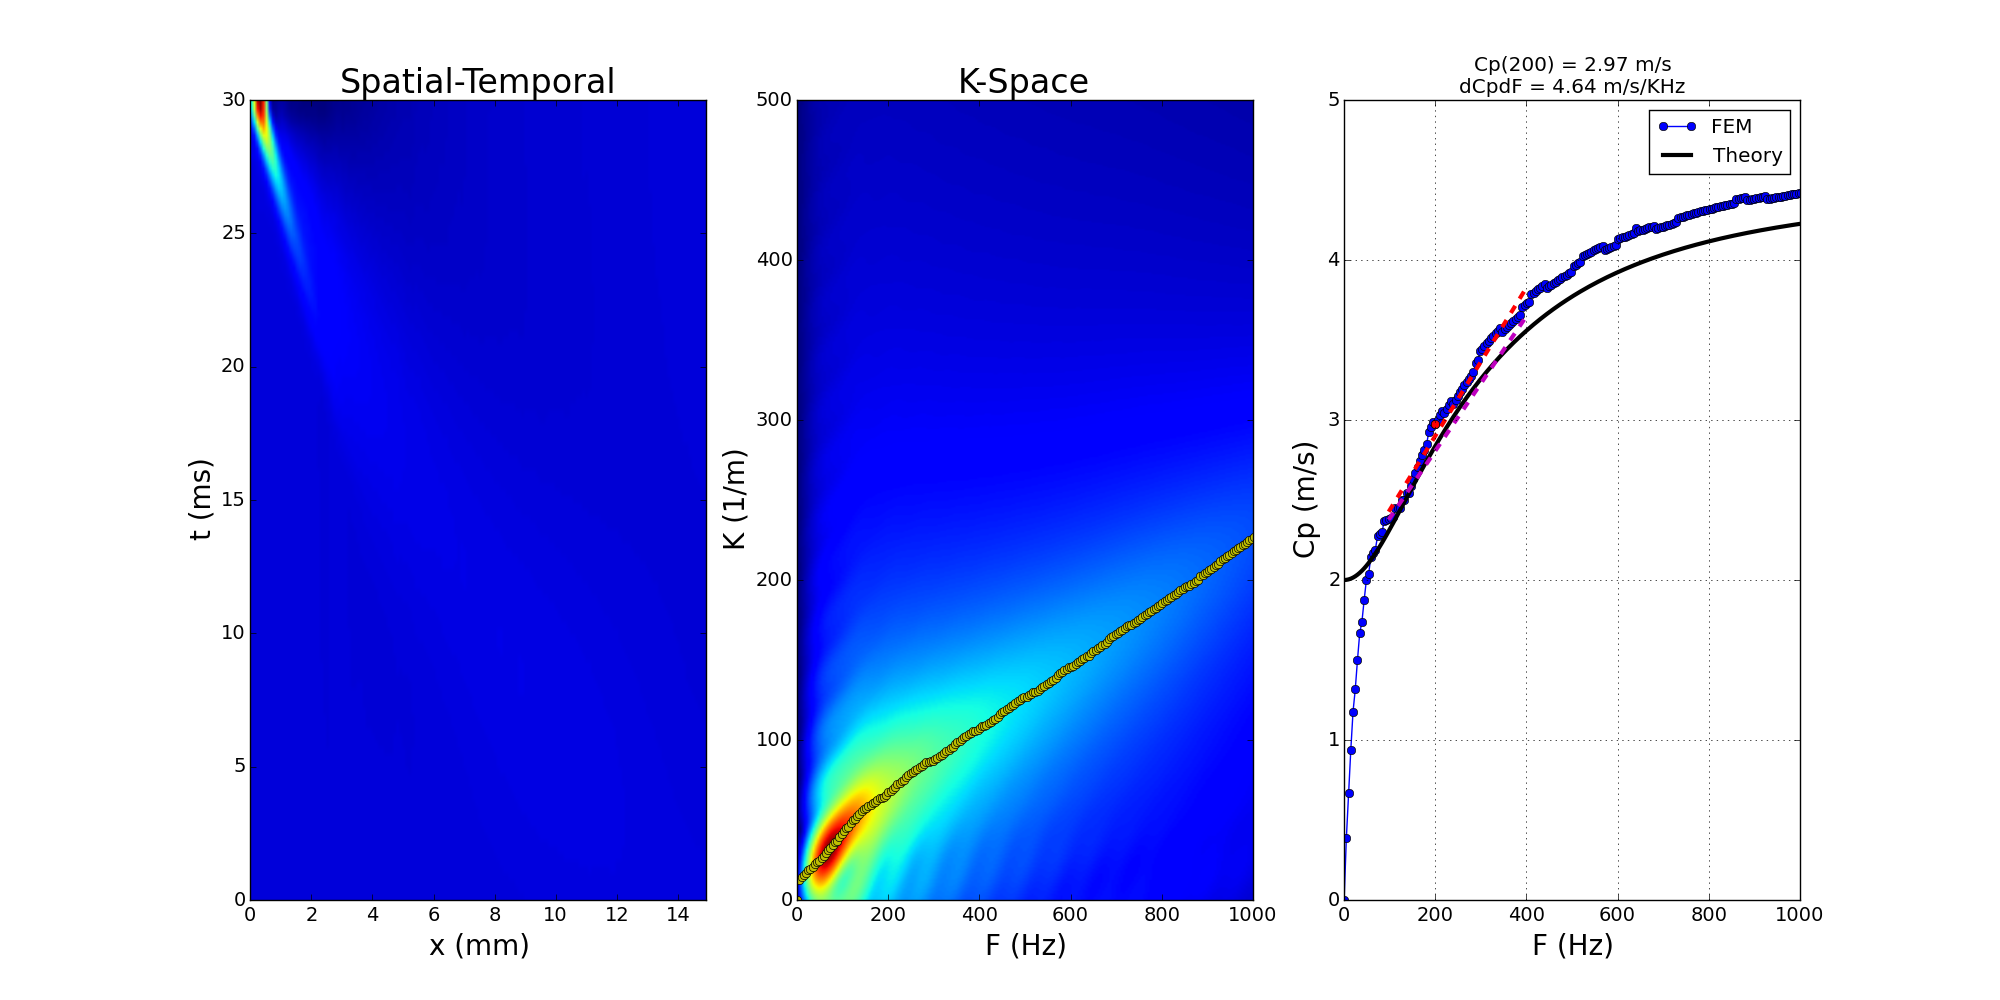
\includegraphics[width=0.75\linewidth]{figs/G020kPa_GI4kPa_BETA4000.png}\\
    \end{tabular}
    \caption{Representative k-space and phase velocity reconstructions 3
        viscoelastic materials that resemble the CIRS Phase II phantoms
        (Figure~\ref{fig:phantom_liver_scatter_plot}).}
\label{fig:ve_data}
\end{figure}


\begin{table}[htb!]
    \centering
    \caption{Viscoelastic material phase velocity metrics compared to theory.
        The phase velocity was calculated at 200 Hz, and the phase velocity
        slope was calculated from 100--400 Hz.  Percent error deviation between
        the FEM-derived metric and the theory are shown in parentheses.}
    \begin{tabular}{|c|c|c|c|c|c|c|}
    \hline
    \multirow{2}{*}{$G_0$ (kPa)} & \multirow{2}{*}{$G_\infty$ (kPa)} & \multirow{2}{*}{$\beta$ (Pa$\cdot$s)} & \multicolumn{2}{c|}{$c$ (200 Hz, m/s)} & \multicolumn{2}{c|}{$\frac{dc}{df}$ ((m/s)/Hz)} \\ \cline{4-7}
            & & & Theory & FEM & Theory & FEM \\ 
            \hline
            10.0 & 2.0 & 6666.7 & 1.71 & 1.78 (+4.1\%) & 2.16 & 2.33 (+7.9\%) \\ \hline
            15.0 & 4.0 & 5500.0 & 2.33 & 2.38 (+2.1\%) & 2.47 & 2.72 (+10.1\%) \\ \hline
            20.0 & 4.0 & 4000.0 & 2.84 & 2.97 (+4.6\%) & 4.21 & 4.64 (+10.2\%) \\
    \hline
    \end{tabular}
\label{table:elastic}
\end{table}
